\section{Non-axisymmetric orbits}

A potential of a non-axisymmetric case with two fixed point
masses is given by:
\begin{equation}
    U(x,y) = -[(x-a)^2 +y^2]^{-1/2} -[(x+a)^2 +y^2]^{-1/2}.
    \label{eq:non-axisymmetric}
\end{equation}

% Although far from obvious, this potential can be separated in confocal
% elliptical coordinates and put in a Staeckel form (as described in B\&T
% and therefore has regular orbits. If the two point masses were in orbit
% around each other, the orbits would not be regular. In other words, the
% real three body problem has chaotic trajectories!
%%%%%%%%%%%%%%%%%%%%%%%%%%%%%%%%%%%%%%%%%%%%%%%%%%%%%%%%%%%%%%%
%=========================SUBSECTION===========================
%%%%%%%%%%%%%%%%%%%%%%%%%%%%%%%%%%%%%%%%%%%%%%%%%%%%%%%%%%%%%%%
% \subsection{}
% (a) Again, pick some initial conditions and integrate the orbits. Just
% to be definite a = 1=2 (although the problem scales with a so you
% can choose value you wanted and get the same results).

By integrating the potential you can find the equations of motions. In this case, they are
\begin{align*}
    F&=-\nabla U(r) =-(\frac{\partial U(r)}{\partial x}+\frac{\partial U(r)}{\partial y}\\
    \Ddot{x}&=-\left[\frac{x-a}{(x-a)^2+y^2}+\frac{x+a}{(x+a)^2+y^2}\right] \\
    \Ddot{y}&=- \left[\frac{y}{(x-a)^2+y^2}+\frac{y}{(x+a)^2+y^2}\right]
\end{align*}


This can be evaluated using the initial conditions listed in table \ref{tab:nonaxisIV} and $a= \frac{1}{2}$.


\begin{table}[]
    \centering
\begin{tabular}{lrrrrr}
\toprule
{} &    x &    y &  $v_x$ &  $v_y$ &   Time \\
\midrule
Orbit 3 & 2.00 & 0.00 &   0.00 &   0.40 & 100.00 \\
Orbit 4 & 2.00 & 0.00 &   0.00 &   0.50 & 100.00 \\
Orbit 5 & 3.00 & 0.00 &   0.00 &   0.60 & 100.00 \\
\bottomrule
\end{tabular}

    \caption{Initial conditions used for the orbits shown in Figure \ref{fig:nonaxisOrbits}.}
    \label{tab:nonaxisIV}
\end{table}

\begin{figure*}[htb!]
    \centering
    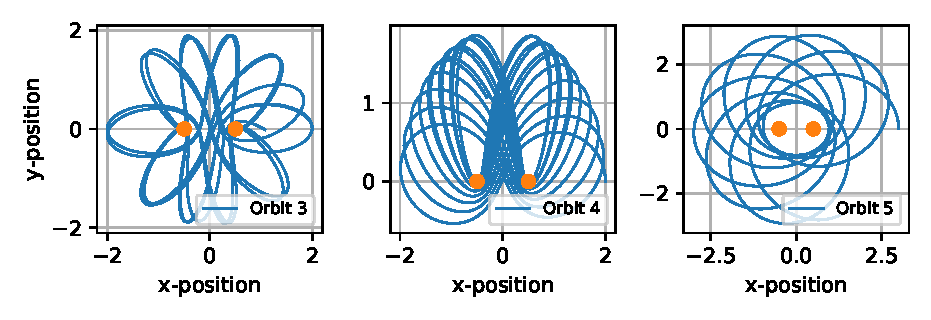
\includegraphics{CodeAndFigures/NonAxisSymetricOrbits.pdf}
    \caption{Orbits of a test particle under non-axisymmetric potential given by \ref{eq:non-axisymmetric} using initial conditions listed in Table \ref{tab:nonaxisIV}.}
    \label{fig:nonaxisOrbits}
\end{figure*}

Figure \ref{fig:nonaxisOrbits} shows three orbits by using Leapfrog integration and the initial conditions listed in Table \ref{tab:nonaxisIV} for \SI{100}{\s}. Orbit 1 and Orbit 2 are considered box orbits while Orbit 3 is a tube orbit. 
Box orbits are orbits that passes close to every point inside a box in the center. 


%%%%%%%%%%%%%%%%%%%%%%%%%%%%%%%%%%%%%%%%%%%%%%%%%%%%%%%%%%%%%%%
%=========================SUBSECTION===========================
%%%%%%%%%%%%%%%%%%%%%%%%%%%%%%%%%%%%%%%%%%%%%%%%%%%%%%%%%%%%%%%
\subsection{}
% (b) There are two different kinds of orbits in this potential: tube orbits
% and box orbits. Box orbits come arbitrarily close to the center of
% force filling a closed area (similar to Lissajous figures). In fact,
% there are two cases of box orbits here: those which come close to
% one and those which come close to both centers of force. Find an
% example of each case.




%%%%%%%%%%%%%%%%%%%%%%%%%%%%%%%%%%%%%%%%%%%%%%%%%%%%%%%%%%%%%%%
%=========================SUBSECTION===========================
%%%%%%%%%%%%%%%%%%%%%%%%%%%%%%%%%%%%%%%%%%%%%%%%%%%%%%%%%%%%%%%
%\subsection{}
% (c) Extra credit Investigate the relationship between conserved quantities and the envelope of the orbits. Report your findings.
% Note: because the force is generated by two point masses, box orbits
% will come arbitrarily close to one or both of the force centers. This
% makes the solution numerically tricky. Consider using small error tolerances and/or small time steps . . .

\clearpage